% Chapter 2

\chapter{Literature Review} % Main chapter title

\label{Chapter2} % For referencing the chapter elsewhere, use \ref{Chapter2} 

\lhead{Chapter 2. \emph{Literature Review}} % This is for the header on each page - perhaps a shortened title

%----------------------------------------------------------------------------------------
% citation - (Bekerian 2005) - ITB
% citation - (Bekerian, 2005) or Bekerian (2005)
%para - \citep{Fiess2002353} - (Bekerian, 2005)
%para - \citet{Fiess2002353} - Bekerian (2005) - default??

% -------- 1. The author(s) and year of publication are cited in the text - \citep - NOTE p ...
% Example  - In conjunction with their perceived low social status, the key factors that influence the use of contraception among African Women are the dominance of the husband in the marriage and his opposition to family planning (Beekle & McCabe 2006).

% -------- 2. The author(s) surname is part of a sentence - \citet (default)
%Example - Findley (2003) suggests that loneliness is rarely considered as appropriate for intervention research; however, the results of such studies are promising.
%Example - Findley (2003) and Wikström (2002) agree that …

Speculators, stock market traders, market participants or simply traders are all terms used to describe individuals and organisations who attempt to make a living from buying and selling various financial assets in a huge range of markets around the world. Clearly the ability to forecast the direction of market movements, up or down, is vital to these individuals and entities. To this end a wide variety of techniques and methods have been tried and used by the participants in the market. Further, over the last few decades academics have shown an interest in this field and attempted to quantify and justify the wide variety of techniques used. 

Two areas where traders and academics have looked for help in predicting future market direction is time series forecasting and the use of technical indicators. This chapter is divided into two these general categories, time series modelling and the use of technical indicators. 


\section{Technical Analysis}

\subsection{Trading Systems}
\label{sec:tradingsystems}
A wide variety of techniques have been employed by financial market traders in their attempts to make profits with the term \textquotedblleft trading system" being applied generally to the methodology used. Often trading systems are \textquotedblleft mechanical" in nature in that traders use a distinct set of rules in order to guide them as when to enter a trade, when to exit and so on. \cite{faith2007way}, one of the original and now famous \textquotedblleft Turtle Traders" provides an excellent overview of mechanical trading systems (and how they were to become known as the \textquotedblleft Turtles"). 

\cite{weissman2005mechanical} makes the point that there are several aspects to a trading system. Firstly there are entry and exit signals, which are market events that trigger a speculator to enter into the market and either buy or sell a particular asset. These signals are typically events such as a fast moving average crossing a slower one, the market hitting a certain price or the occurrence of a particular chart pattern (see section \ref{sec:candlesticks}). Other elements of a trading system include position sizing rules and money management strategies such that returns are significant, losses are minimised and the entire risk profile is controlled.

Many traders erroneously mistake entry and exit signals as being a full trading system in themselves whereas in actuality they are merely components of a system \citep{beau1999day}. Likewise most, if not all, papers published by academia focus on entry and exit signals alone, which is probably a result of several factors. Firstly, entry and exit signals are important components in  trading systems and are a good place to start in system development. Additionally, the other aspects of a system are not as well known and their importance is often ignored \citep{kaufman2013trading}. Finally, testing an \textquotedblleft entire" system as defined here is far more difficult and time consuming than considering entry and exit signals alone and often it is not practical to extend a study to include a full system. In summary there is value in considering entry and exit signal in isolation but one has to remember it is not the whole story.

Attempting to forecast stock market prices is a complex and challenging endeavour, yet one that is widely encountered. There is a large body of research published in this area which has been reviewed by \cite{Atsalakis20095932}. Work usually focuses on either individual stocks or more commonly stock indices. Stock indices are the sum movements of many individual equities and therefore reflect the movement of the market as a whole as opposed to any one stock. Many stock market indices have been investigated including those belonging to well-developed countries such as those in Western Europe, North America etc.\ as well as developing markets such as those in eastern Europe.

In trying to predict stock market movements a variety of input variables have been used. Frequently, the so-called OHLC (open, high, low and closing prices) are used as inputs along with a variety of technical indicators \citep{Fiess2002353}. In addition many authors have used a combination of markets, for example \cite{Huang20052513} use both the USD/YEN exchange rate and the S\&P 500 to build a prediction model for the Japanese NIKKEI index. A variety of predictive methodologies have been reported in the literature including linear and multi-linear regression, ARMA and ARIMA models, genetic algorithms (GAs), artificial neural networks (ANNs), random walk (RW) and the so-called buy and hold (B \& H) strategy.

A variety of performance measures have been reported including both non-statistical and statistical methods. Non-statistical performance measures used include annual return and annual profit of a particular model as well as the hit rate or the number of times a model correctly predicts whether a market will go up or down. Alternatively a variety of statistical measures have also been employed and prominent amongst them are, mean absolute error (MAE), root mean squared (RMSE), mean squared prediction error (MSPE), correlation coefficient and autocorrelation squared correlation and Akaike’s minimum final prediction error (FPE).

%Simple Technical Trading Rules and the Stochastic Properties of Stock Returns - \cite{Brock} - IMP PAPER
Two well studied and used methodologies in stock trading are the moving average system and range breakout system reported by \citep{Brock} in one of the very earliest papers published covering technical analysis. In a moving average system (see section \ref{sec:Chp4a:sma}) the speculator buys a market when its price is above the moving average and sells in the reverse situation. A large number of variations on this theme can be found, with the use of two moving averages being popular. When using two averages there is normally a \textquotedblleft fast" one, usually of the order of 10 to 25 days,  and a \textquotedblleft slow" one in the 50 to 250 day range. In these circumstances a buy is usually triggered when the fast average crosses above the slower average. The theory is that the moving averages follow the trends in the market and thus allow the market participant to trade in the direction of the trend, which is an advantageous situation for the trader.

A second popular idea is that of breaking out of a range. Often financial markets trade between a range of values in a particular time period, essentially markets are either trending (up or down) or not trending at all but moving within a defined range. While moving in a range the lower price boundary is referred to as support and the upper one as resistance. In a breakout system the analyst buys a market when it moves beyond these resistance levels or sells when it breaks below the support. \cite{Brock} analysed both these two ideas and found merit in them. Using daily data from the Dow Jones industrial index they found that these strategies provided better results than those generated with random walk, AR and GARCH models.

%\subsection{Data}
%1. Towards the fundamentals of technical analysis: analysing the information content of High, Low and Close prices - \cite{Fiess2002353}
%\begin{itemize}
%\item \textquotedblleft Candlestick analysis is a popular form of TA that combines Open, High, Low and Close prices for the purpose of charting and forecasting "
%\item \textquotedblleft the difference between Open and Close prices serves as a measure of the direction and the extent of intradaily trends. 
%\item \textquotedblleft The difference between High and Low prices marks the intradaily trading range and represents a measure of volatility. 
%\item \textquotedblleft For many forms of TA, it is the interaction between trend and volatility that is assumed to be informative about future price developments.
%\end{itemize}

%11. Candlestick technical trading strategies Can they create value for investors - \cite{Marshall20062303}
% nice section on why Dow Jones ...

%\subsection{Time Periods}
%2. Profitability of technical stock trading - has it moved from daily to intrday data? - \cite{Schulmeister2009190}
%\begin{enumerate}
%\item looking time frames - day vs 30 mins
%\item - trend following and contrarian
%\item - sma and RSI - kaufman
%\end{enumerate}


\subsection{Technical Analysis Overview}
Technical analysis is the technique of looking at the past history of a financial market, identifying patterns and trends and utilising the information in predicting future price movements \citep{bulkowski2011encyclopedia}. A technical indicator is a method used to identify a particular pattern, and there have been a large number developed over the years to predict situations such as the start of a trend or a reversal in price movement.  A wide range of papers on technical analysis (TA) indicators and methods can be found in the literature. Likewise technical analysis is prominent in many best selling books including Market Wizards \citep{schwager2012market}, New Market Wizards \citep{schwager2012new} and Covel's Trend Following \citep{covel2009trend}. In the following sections various technical indicators are introduced and their use in predicting market movements are explored. Firstly, the question of whether technical analysis even works is addressed, as this has received attention in the literature \citep{Marshall2005,Reitz2006121,Schulmeister2009190,Marshall2008199}.  Although technical analysis is widely used in the market place there is a question mark over the entire concept behind it and many people, especially academics, are highly sceptical about the validity of the entire approach.

\subsection{Does Technical Analysis Work?}

\cite{Friesen20091089} have examined various price "patterns" used by traders in their systems such as \textquotedblleft head-and-shoulders” and \textquotedblleft double-top” patterns. The authors note that although a wide array of patterns have been identified and documented there lacks any convincing explanations for the formation of these patterns and how they can lead to profitable trading systems.  The authors report that several studies based on the US equity market have identified distinct behaviours, namely the tendency for short-term momentum over 1 year to 6 months \citep{Bondt,chopra1992,jegadeesh1993}, longer term mean reversion and finally price reversals over the one to four week period \citep{jegadeesh1990,lehmann1990,jegadeesh1995,kelley2008}. These observations lend support to the success of trading systems that purport to detect and follow trends in the market \citep{sweeney182,levich1993,neely1997,Dueker2007}.

The authors present a model that can explain the profitability of selected trading rules that utilise past chart patterns. One important aspect of this model is the inclusion of confirmation bias, which shows up in a wide range of decision making processes. Their model displays negative autocorrelations over the very short term, positive ones in the
mid term and become negative again over the longer horizon, reflecting the documented empirical properties of US stock prices.  It is suggested that traders take market positions affected by their original biased view which leads to autocorrelations and price movement patterns resulting in the previously described market behaviour.

\cite{Shynkevich2012193} investigated the power of a large selection of technical trading rules to yield profits when applied a selection of small cap and technology portfolios (US stocks) between 1995 and 2010. The author chose technical indicators from four general categories:
\begin{enumerate}
\item standard filter rules - for example a buy is generated when prices increase from a previous low. Such a low may be defined as the lowest closing price in a particular period. In more recent years this technique has been replaced by moving averages. 
\item  moving averages - signals generated when short MA cross long MA. 
\item  support and resistance trading strategy (SR) - a buy is initiative when prices rise above a local maximum, and vice versa for a local minimum price.
\item  Channel breakout - related to SR, a buy/sell is triggered when a price moves outside a channel generated from highs and lows of a certain period.
\end{enumerate}
The author applied a variety of parameters in each model resulting in a total of 12937 models being tested. It was reported that TA produced positive results in the first half of the time period tested, but not in the latter half. In the second half of the time period studied TA provided inferior performance than a buy-and-hold approach, i.e. a trader simply buys a particular asset and waits. The author concludes these differences in performance are due to equity markets having become more efficient in recent years which has reduced the short term predictive powers of TA.

The use of technical analysis in the finance community was studied by \cite{Menkhoff20102573} who looked into its use by professional fund managers. This study is note worthy as it used data from experienced and educated market professionals and not a wider cross-section of traders. With the advent of the internet and the explosive growth in on-line financial charting and trading sites, financial  trading became accessible to the general public, resulting in huge numbers of amateur traders entering the market. All of the web sites that cater for this segment of traders offer a huge number of technical analysis indicators built into their respective charting packages and even a rudimentary visit to any of the discussion forums will demonstrate the popularity and wide spread use of technical analysis. 
 
The author surveyed 692 fund managers in several countries, with funds of various sizes under management. The vast majority of these fund managers reported using technical analysis to some degree and particular faith was put in TA for predicting price movements in the short term of up to a few weeks, beyond which focus shifts to fundamental analysis. Further, the workers found that smaller asset manager firms make greater use of TA, possibly because deriving the information for fundamental analysis is beyond their resources. Finally, most respondents to the survey believe that human psychology is the reason TA works. In particular they suggest psychological biases in the market participants are the root cause of market trends and that TA is able to identify and follow them.

%9. Is technical analysis profitable on a stock market which has characteristics that suggest it may be inefficient? - \cite{Marshall2005384} - TA doesn't work - couldn't download.
%
%10. On the predictive content of technical analysis - \cite{Reitz2006121}
%TA does work, an explanation why ...
%
%12. Dangers of data mining: The case of calendar effects in stock returns - \cite{Sullivan2001249}
%\textquotedblleft The common practice of using the same data set to formulate and test hypotheses introduces data-mining biases that, if not accounted for, invalidate the assumptions underlying classical statistical inference"  Calendar events not significant.
%
%
%16. Does intraday technical analysis in the U.S. equity market have value? - \cite{Marshall2008199}
%This paper investigates whether intraday technical analysis is profitable in the U.S. equity market. Surveys of market participants indicate that they place more emphasis on technical analysis (and less on fundamental analysis) the shorter the time horizon; however, the technical analysis literature to date has focused on long-term technical trading rules. We find, using two bootstrap methodologies, that\textbf{ none of the 7846 popular technical trading rules we test are profitable after data snooping bias is taken into account}. There is no evidence that the market is inefficient over this time horizon.

\subsection{Moving Average Indicators}
%5. Drivers of tech trend-following rules profitability in world stock markets - \cite{Prodan2013214}
A study of moving average convergence divergence (MACD) is reported by \cite{Prodan2013214}. MACD is a technique which attempts to detect the early stage of a trend as it forms, and is widely used by market participants. It is described in more detail in Appendix \ref{AppendixB} section \ref{appB:MACD}. \cite{Prodan2013214} apply MACD to a wide range of national stock market indices comprising developed as well as emerging markets. The authors compare the MACD signals against entry signals generated from simple break out systems (described previously). The comparison systems would generate a buy signal if the price moved higher than a moving average (MA), set at either 22, 56 and 200 days. The MACD and the comparison system using 22 day moving averages are classified as short horizon signals, while the break out of the 56 and 200 day MA are considered long horizon signals. The workers reported that the MACD indicators provide for profitable returns on 23 of 30 national indices, but that the 22 day MA performs better being positive in 27 of the 30 markets.

%------------------LOOK at this again -----------
%
%%7. An asset allocation perspective on the use of moving averages - \cite{Zhu2009519}
%An alternative use of moving averages is described by \cite{Zhu2009519}. They describe the use of moving averages in the problem of allocating funds appropriately between assets in a portfolio. It is reported that the use of MA in conjunction with fixed rules can enhance returns in comparison to the fixed rule alone. The workers claim that using the porfolio theory from \cite{Markowitz} or the theory of two fund separation from \cite{Tobin} in combination with MA, a theoretical basis exists which explains the improved returns when combining either theorem in combination with MA.
%
%------------------------------------------------

\subsection{Candlesticks Patterns}
\label{sec:candlesticks}
Probably the oldest form of technical analysis in use today is the so-called candlestick analysis, so named because daily open and close prices are plotted such that they resemble candlesticks \citep{morris2006candlestick}. Figure \ref{fig:Candlestick} is an example of daily prices being plotted as a candlestick, this plotting method is today ubiquitous in trading software. Typically the colour in which the candlestick is plotted indicates whether the price went up or down over the course of the day. Many charts that are plotted in colour use green to represent days that close up and red for days that close down. The main body of the candlestick represents the movement from open to close, and the protruding lines mark the high and low of the day.

\begin{figure}[tbph!]
\centering
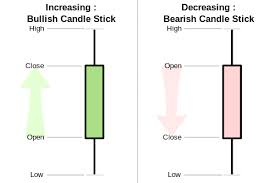
\includegraphics[width=7cm]{chp2_Candlestick}
%\caption{fs yrytrytr}
\caption[Candlestick representation of daily open and close prices]{Candlestick representation of daily open and close prices. Different colouring is used to distinguish between prices going up or down.}
\label{fig:Candlestick}
\end{figure}

Technical analysis via candlesticks is reputed to have been developed by Munelusa Homma, a legendary trader of rice in Osaka, Japan who made a fortune analysing rice prices with candlesticks in the seventeenth century \citep{nison2001japanese}. Candlestick patterns with supposed predictive qualities can be derived from a single day or from considering a few days, usually 2 or 3, together \citep{bigalow2011profitable}. There are a huge number of patterns recorded in the literature and usually assigned exotic names such as \textquotedblleft White Marubozu", "Black Shooting Star" and "Hanging Man". Examples of such named patterns can be seen in Figure \ref{fig:Candlestick_Patterns}.

\begin{figure}[tbph!]
\centering
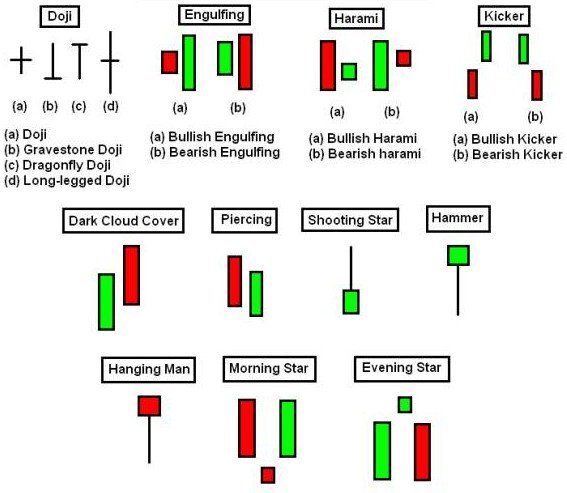
\includegraphics[width=9cm]{chp2_Candlestick_Patterns}
\caption[Examples of well known candlestick patterns]{Examples of well known patterns encountered in candlestick analysis.}
\label{fig:Candlestick_Patterns}
\end{figure}

Candlestick patterns are essentially visualisation tools providing an easy to comprehend view of the market movements in a particular day. However there is some vital information which is not conveyed in a candlestick. In particular the order of events isn't displayed. Figure \ref{fig:chp2_candle_order} shows how two days can produce the same candlestick but in actuality the price movements and volatility in them was very different. Depending upon the type of trading system being employed this could have important effects.

\begin{figure}[tbph!]
\centering
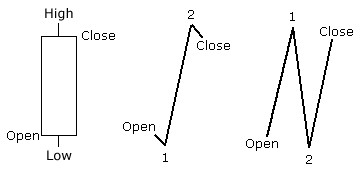
\includegraphics[width=7cm]{chp2_candle_order}
\caption[Candlesticks and market movement]{Candlesticks don't provide information regarding the order of price movements. Both these daily price movements would be represented with the same candlestick pattern.}
\label{fig:chp2_candle_order}
\end{figure}


%11. Candlestick technical trading strategies Can they create value for investors - \cite{Marshall20062303}
As always with technical analysis there is doubt as to the validity of the methods despite its almost universal employment. An in-depth study of the predictive power of a range of candlestick patterns on stock prices between 1992 and 2002 from the Dow Jones Industrial Average (DJIA) was carried out by \citep{Marshall20062303} in which doubt was cast on the validity of candlestick patterns to predict market movements. The workers used a range of bullish (signals that indicate a trader should buy) and bearish (signals that indicate a trader should sell) candlestick patterns to initiate trades on the various stocks. Trades were held for ten days as it was assumed that these patterns reflect short terms trends and thus have a predictive power in a similar time frame. In order to quantify the results generated from the use candlestick patterns they were compared to results observed from four alternative null models. Simulated stock data was generated using a bootstrapping methodology \citep{EfronBootstrapping} and then four null models were applied to the data, random walk, an autoregressive process of order one (AR(1)), a GARCH in-Mean (GARCH-M) model and an Exponential GARCH (EGARCH) model.

From the comparison of the results generated from the candlestick patterns and the four null models the workers concluded that the variety of candlestick patterns tested had no predictive power on the stocks at all. The returns from making buying and selling decisions based on candlestick patterns didn't outperform the null models on the simulated data. As always one has to be slightly careful with results of this nature as the trading period was fixed at ten days, in other words the candlestick patterns were used as an entry signal for the trade but there wasn't an exit signal. Further in reality use of candlesticks analysis would be incorporated into a trading system, which typically consists entry and exit signal, position sizing rules and money management strategies \citep{faith2007way}.

\subsection{Trend Reversal Oscillators}
%6. Adaptive use of technical indicators for the prediction of intra-day stock prices - \cite{TanakaYamawaki2007125}
\cite{TanakaYamawaki2007125} reported the use of several technical analysis techniques in the successful prediction of price movements in eight stocks found on the New York Stock Exchange (NYSE) by analysing tick data. The predictions were in the very short term as tick data is the most granular level reported in financial data. The workers used ten technical analysis indicators from three broad classes, namely trend indicators, oscillators to find market reversals and momentum indicators to measure the strength of the market. Combinations of indicators, typically from the different categories are usually combined by market participants into a variety of systems. In this study the ten indicators can form a possible 1023 combinations. A genetic algorithm was used to determine the best combination of indicators for each stock, resulting in a customised combination for each. Using each stock's indicators, the next ten ticks of data were modelled with very high accuracy, with predictions for IBM's stock being the best at a very impressive up to 82\%. 

%13. "Intelligent stock trading system based on improved technical analysis and Echo State Network " - \cite{Lin201111347}
%MA, RSI, ROC, stochastics, candle's, - INTERESTING

%14. "Is technical analysis profitable on a stock market which has characteristics that suggest it may be inefficient" - \cite{Marshall2005384}
%NZ Stock mkt - MA, ROC, 

%\subsection{Data Snooping}
%17. The impact of data snooping on the testing of technical analysis: An empirical study of Asian stock markets - \cite{Chen2009580}
%The primary aim of this study is to investigate the validity and predictability of technical analysis in eight Asian equity markets. We employ the bootstrap tests of White (2000) and Hansen (2005) to determine whether any superior trading rule is found to exist amongst the 'universe' of technical trading rules identified by Sullivan et al. (1999). We use these powerful bootstrap tests to ascertain the profitability of technical analysis, along with two institutional adjustments for non-synchronous trading and transaction costs. The empirical results indicate that these three elements, data snooping, non-synchronous trading and transaction costs, have significant impact on the overall performance of technical analysis; indeed, the results for these eight Asian stock markets support the efficient market hypothesis, demonstrating that the generation of economic profits through the use of technical analysis is \textbf{extremely unlikely} with these particular markets.
%
%Earlier paper - \cite{Prodan2013214}

\section{Time Series}
%19 - 25 years of time series forecasting - \cite{DeGooijer2006443}
The study of forecasting time series data has been an active area of study for several decades and an overview of work over 25 years has been documented by \cite{DeGooijer2006443}. Series data is ordered such that the ordering is an important if not critical aspect of the data and the requirement to maintain this ordering enforces certain requirements on its processing. Series data can be ordered by factors such as distance or height but typically time is the ordering encountered, and thus such collections are referred to as time series. Analysis of time series data is found in a wide range of areas including, Sales Forecasting, Speech Recognition, Economic Forecasting, Stock Market Analysis, Process and Quality Control and Seismic Recordings.

In general with non-series data we are interested in the relationships between the attributes of any particular row of data and perhaps how they affect the parameter we are interested in. Frequently some kind of regression technique is used in this kind of analysis in order to answer questions such as how is rainfall in an area affected by altitude or how does fuel consumption vary with car engine size \citep{han2011data}.

However with time series data there is an additional consideration, the relationship between the attribute's current value to that of its previous or later values. This is known as auto-correlation \citep{mills2011} and more details can be seen in section \ref{sec:autoregression}. Typically with financial data we are interested in previous values, in other words how is today's closing price affected by the closing prices one, two or three days ago?

As illustrated in Figure \ref{fig:TimeSeriesComponents} a time series can contain some or all of the following components:
\begin{enumerate}
\item Trend - the overall direction of the series, is it increasing or decreasing over time?
\item Seasonality - regular variations in the time series that is caused by re-occurring events, for example a spike in sales during the Christmas period \citep{So2014212}.
\item Random component - additional fluctuations in the series that may be attributed to noise or other random events.
\end{enumerate}

\begin{figure}[tbph!]
\centering
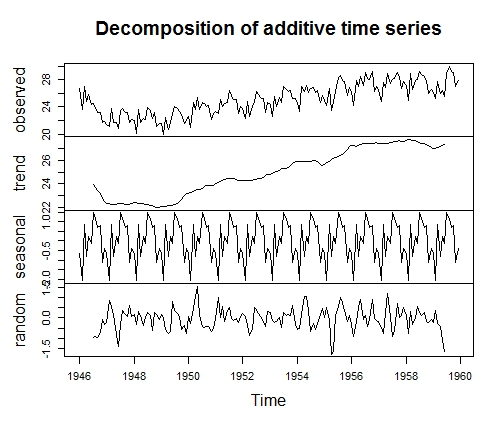
\includegraphics[height=12cm]{chp2_TimeSeriesComponents}
\caption[A time series decomposed into primary components]{A time series decomposed into its three primary components.}
\label{fig:TimeSeriesComponents}
\end{figure}

There are three primary types of time series, stationary, additive and multiplicative. Stationary series have constant amplitude without a trend element and an example can be seen in Figure \ref{fig:Stationary_ts}. Often stationary time series are repetitive, in other words showing constant auto-correlation and are considered the easiest type to model. A stationary time series can be composed of a seasonal element and/or a random component, thus:

\begin{center}
\textit{stationary time series = seasonality +/or noise}
\end{center}

\begin{figure}[tbph!]
\centering
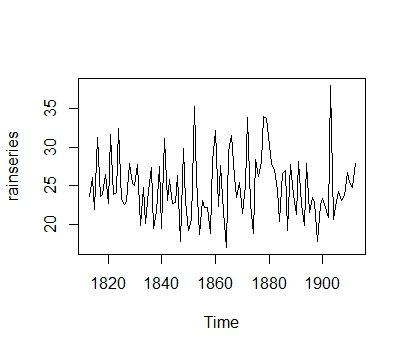
\includegraphics{chp2_Stationary_ts}
\caption[A stationary time series]{Example of a stationary time series which can be made up from noise and/or a seasonal component.}
\label{fig:Stationary_ts}
\end{figure}

The second type of time series is the additive type. In this type all three components of the series are present, trend, seasonality and noise. The distinguishing feature here is the amplitude of the seasonal component in that it is quite regular being static over time. An example of an additive series can be seen in Figure \ref{fig:Add2_ts}. This time series is trending upwards overall but there is a clear repetitive pattern of peaks and troughs caused by the seasonality, with the heights of the peaks all being similar. We can consider an additive time series as:

\begin{center}
\textit{additive time series = trend + seasonality + noise}
\end{center}

\begin{figure}[tbph!]
\centering
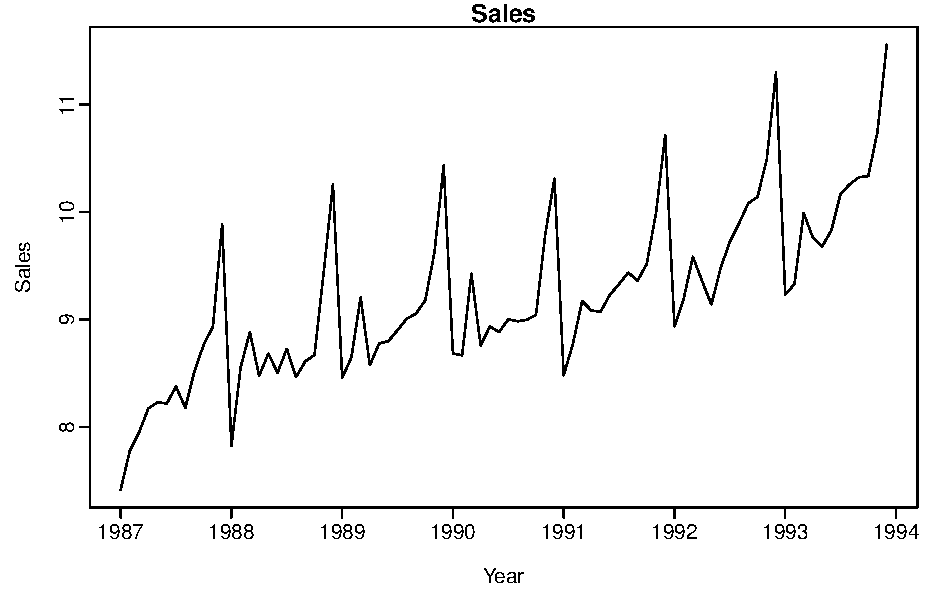
\includegraphics{chp2_Add2_ts}
\caption[An additive time series]{Example of an additive time series which results from all three components trend, noise and seasonality.}
\label{fig:Add2_ts}
\end{figure}

The third type of time series, as seen in Figure \ref{fig:Multi_ts} is multiplicative. This is similar to the additive version except the amplitude of the seasonality increases over time. It can be considered as:

\begin{center}
\textit{multiplicative time series = trend * seasonality * noise}
\end{center}

\begin{figure}[tbph!]
\centering
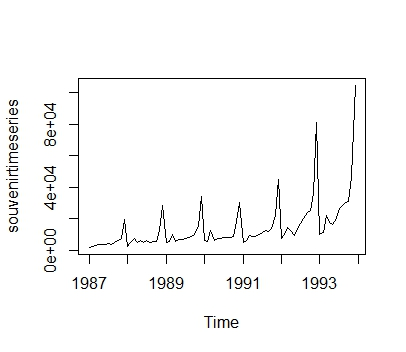
\includegraphics{chp2_Multi_ts}
\caption[A multiplicative time series]{Example of a multiplicative time series resulting from the effects of trend, noise and seasonality.}
\label{fig:Multi_ts}
\end{figure}

Financial time series can be considered as containing all three elements of a time series. They can show properties of a stationary time series when they are range bound and only move between two values. At other times, markets trend strongly consistently, making new highs or lows and exhibit properties of an additive and occasionally a multiplicative series.

\subsection{Time Series Smoothing}
\label{sec:expsmoothing}
Smoothing is an important and widely adopted method to predict financial markets.  Recent work on smoothing time series data has its origins in \cite{brown1959statistical}, \cite{brown1963statistical}, \cite{Holt20045} and \cite{Winters1960}. Typically, the various smoothing techniques encountered are based around the concept of moving averages. This section will introduce a variety of smoothing methods commonly encountered in forecasting financial data. 

\subsubsection{Simple Moving Average (SMA)}
\label{sec:chp2_sma}
A simple moving average is calculated from the value itself and its neighbours, which can be ahead or behind in the series. In this study values behind the current value are considered. The number of previous values included is often referred to as the \textquotedblleft window", so if one was to consider the current value and four previous ones this would be considered a simple moving average of lag 5 (SMA5). An example of a simple moving average can be seen in Table \ref{tab:SMA}, where a SMA5 of the closing price has been added.

% Table generated by Excel2LaTeX from sheet 'Pairs'
\begin{table}[htbp]
  \centering
  \caption[Example of a Simple Moving Average]{Example of a simple moving average of the closing price with a lag of 5 periods.}
    \begin{tabular}{@{\extracolsep{5pt}}lccccc}
    \toprule
    \textbf{Date} & \textbf{Open} & \textbf{High} & \textbf{Low} & \textbf{Close} & \textbf{SMA5} \\
    \midrule
    02/01/14 & 9598  & 9621  & 9394  & 9400  &  NA \\
    03/01/14 & 9410  & 9453  & 9368  & 9435  &  NA \\
    06/01/14 & 9419  & 9469  & 9400  & 9428  &  NA \\
    07/01/14 & 9446  & 9519  & 9417  & 9506  &  NA \\
    08/01/14 & 9513  & 9516  & 9468  & 9498  & 9453 \\
    09/01/14 & 9492  & 9550  & 9403  & 9422  & 9458 \\
    10/01/14 & 9474  & 9530  & 9441  & 9473  & 9465 \\
    13/01/14 & 9498  & 9519  & 9457  & 9510  & 9482 \\
    \bottomrule
    \normalsize 
    \end{tabular}%
  \label{tab:SMA}%
\end{table}%

\subsubsection{Weighted Moving Average (WMA)}
A simple moving average assigns equal importance to all data points being averaged, however if this is considered unsuitable a higher weighting can be applied to certain data points elevating their importance in the average and thus generating a weighted moving average \citep{WMA2}. Typically the more recent data points in a time series would be given higher importance. One common version of a WMA is to decrease the weighting by one for each period in the average. The formula for calculating a weighted moving average is:

\[ ((n*P_{n}) + (n-1*P_{n-1})+ ... (n-(n-1)*P_{n-(n-1)})) \div (n + (n-1) + ... n-(n-1))\]

where: \\
$ n $ = the number of periods used in calculating the moving average \\
$ Pn $ = the price of the most recent period used to calculate the moving average 

An extra column has been added to the data in Table \ref{tab:SMA} which contains the WMA for the last five close values. The current value was multiplied by 5, the previous one by 4, the previous one to that by 3 and so on. These five values were added together and divided by 5+4+3+2+1 to generate the WMA as shown in Table \ref{tab:WMA}.

% Table generated by Excel2LaTeX from sheet 'Pairs'
\begin{table}[htbp]
  \centering
  \caption[Example of a Weighted Moving Average]{Example of a weighted moving average.}
    \begin{tabular}{ccccccc}
    \toprule
    \textbf{Date} & \textbf{Open} & \textbf{High} & \textbf{Low} & \textbf{Close} & \textbf{SMA5} & \textbf{WMA5} \\
    \midrule
    02/01/14 & 9598  & 9621  & 9394  & 9400  &  NA   & NA  \\
    03/01/14 & 9410  & 9453  & 9368  & 9435  &  NA   & NA \\
    06/01/14 & 9419  & 9469  & 9400  & 9428  &  NA   & NA \\
    07/01/14 & 9446  & 9519  & 9417  & 9506  &  NA   & NA \\
    08/01/14 & 9513  & 9516  & 9468  & 9498  & 9453  & 9471 \\
    09/01/14 & 9492  & 9550  & 9403  & 9422  & 9458  & 9461 \\
    10/01/14 & 9474  & 9530  & 9441  & 9473  & 9465  & 9466 \\
    13/01/14 & 9498  & 9519  & 9457  & 9510  & 9482  & 9481 \\
    \bottomrule
    \end{tabular}%
  \label{tab:WMA}%
\end{table}%

\subsubsection{Exponential Moving Average (EMA)}
An exponential moving average (EMA) is an extension of the weighted moving average \citep{Ord20041}. In comparison to the simple moving average, greater emphasis is given to the most recent data points and the resulting averaged values are closer to the actual observations of the data set. Weighting factors decay exponentially resulting in the emphasis falling on the recent values though not discarding the older ones totally. See Appendix \ref{AppendixB} for full details.

\subsubsection{Moving Averages in Practical Use }
Moving averages are widely used in the financial world to predict the start of trends which is important as trends are considered the best opportunity to make profits from the markets. By their nature moving averages are lagged indicators in that they reflect market action from the past (recent or distant depending on the lag variable) and this can be considered a drawback. The lag period offers a trade off in terms of prediction. If the lag is short and/or weighting is applied the average is affected strongly by recent prices and trends can be detected in the early stages and trading profits can be enhanced. However when the average is close to the current price they have a tendency to generate \textquotedblleft false signals" (see section \ref{sec:tradingsystems} for an explanation of entry and exit signals), in other words prices may start to rise (or fall) but they are not actually in a trend, it is just the natural wax and wane of the market, and traders are said to be \textquotedblleft whipsawed". When the lag variable is long a different problem is encountered. For example, if a price moves above a long moving average the indicated trend is usually genuine, however by the time this is reflected in the average a lot of the trend has developed and the trader has lost a lot of potential profits. Thus there are pros and cons associated with using the different types of moving average.

\subsubsection{Holt-Winters Smoothing Models}
\label{sec:holtwinters}
The exponential smoothing of a time series containing noise, trend and seasonality was developed by \cite{Winters1960} who as a student of Holt, built upon his previous work, and is today called the Holt-Winters method. This method defines three parameters alpha, beta and gamma which define the degree of smoothing to be applied to the three components of the time series. Firstly, a value of alpha is used to dictate the amount of smoothing to apply, with high smoothing factors placing more emphasis on recent data points at the expense of those further away. In a data set with trend this simple exponential moving average doesn't perform well and a second order of smoothing is needed, so called \textquotedblleft double exponential smoothing". The parameter beta in Holt-Winters defines this second order smoothing. Finally if a seasonal component is also present in the data set a third level of smoothing is introduced making the process a triple exponential smoothing. It is this third level of smoothing that the parameter gamma refers to. Depending upon the nature of the time series one, two or all three of the parameters may be defined in the Holt-Winters methodology.

If researching a time series with no seasonality or trend use of the Holt-Winters model with the beta and gamma parameters set to false, in other words not used, is appropriate. Figure \ref{fig:HW1a} shows the addition of an exponential smoothing line to the stationary data set introduced in Figure \ref{fig:Stationary_ts}.

%\begin{figure}[tbph!]
%\centering
%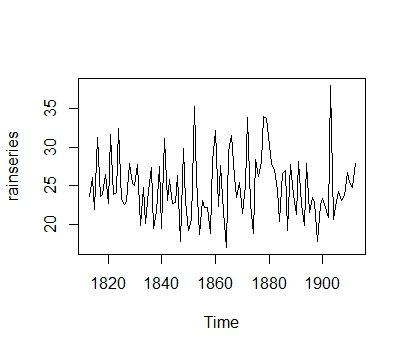
\includegraphics[width=8cm]{chp2_HW1}
%\caption[A time series with no seasonality or trend]{For a time series with no seasonality or trend, the use of Holt-Winters exponential smoothing with the beta and gamma parameters set to false is appropriate.}
%\label{fig:HW1}
%\end{figure}

\begin{figure}[tbph!]
\centering
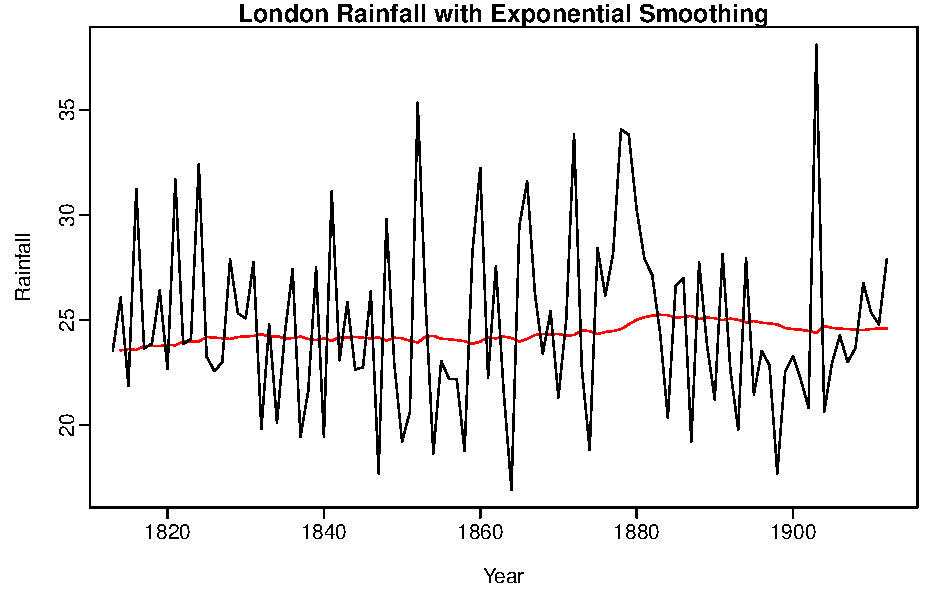
\includegraphics{chp2_HW1a}
\caption[Exponential smoothing of a time series with no seasonality or trend]{A time series with no seasonality or trend, showing the fitted line generated from Holt-Winters exponential smoothing with the beta and gamma parameters set to false.}
\label{fig:HW1a}
\end{figure}

If the time series is additive with a trend but without seasonality the use of Holt-Winters with values used for alpha and beta but with the gamma parameter set to false is appropriate. Such a time series can be seen in Figure \ref{fig:HW2a} with the exponential smoothing. Finally if the time series contains all three components a smoothing line can be fitted using Holt-Winters exponential smoothing in which there are values for all three terms alpha, beta and gamma. Figure \ref{fig:HW3a} is an example of a time series with both trend and seasonality and overlaid with Holt-Winters smoothing generated by using values for all three terms in the smoothing algorithm.

%\begin{figure}[tbph!]
%\centering
%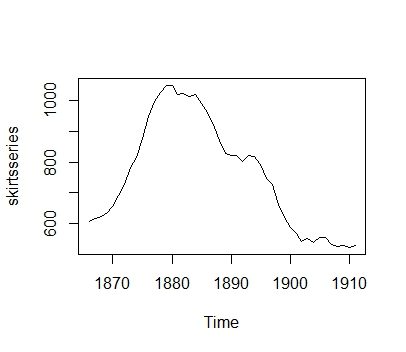
\includegraphics[width=8cm]{chp2_HW2}
%\caption[A time series with trend though no seasonality]{For a time series with trend but no seasonality, the use of Holt-Winters exponential smoothing with the gamma parameter set to false is appropriate.}
%\label{fig:HW2}
%\end{figure}

\begin{figure}[tbph!]
\centering
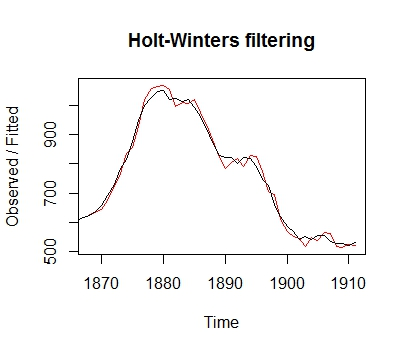
\includegraphics{chp2_HW2a}
\caption[Exponential smoothing of a time series with trend though no seasonality]{A time series with trend though no seasonality, showing the fitted Holt-Winters exponential smoothing with the gamma parameter set to false.}
\label{fig:HW2a}
\end{figure}

%\begin{figure}[tbph!]
%\centering
%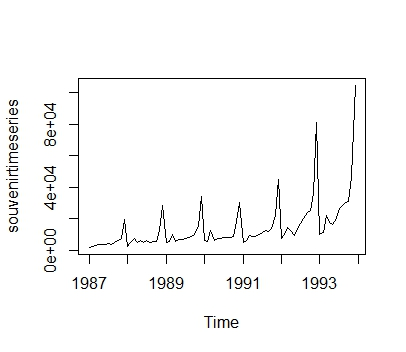
\includegraphics[width=8cm]{chp2_HW3}
%\caption[A time series with trend and seasonality]{For a time series with trend and seasonality, the use of Holt-Winters exponential smoothing is appropriate.}
%\label{fig:HW3}
%\end{figure}

\begin{figure}[tbph!]
\centering
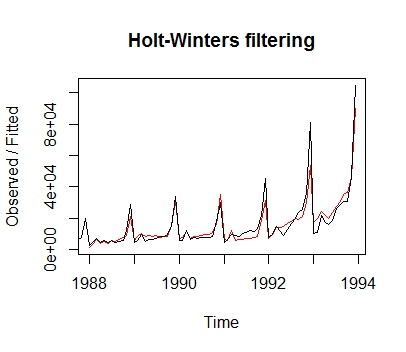
\includegraphics{chp2_HW3a}
\caption[Exponential smoothing of a time series with trend and seasonality]{A time series with trend and seasonality, showing the fitted Holt-Winters exponential smoothing.}
\label{fig:HW3a}
\end{figure}


%%29 - Holt’s exponential smoothing and neural network models for forecasting interval-valued time series " - \cite{Maia2011740}

\subsection{Auto-Regression Family of Models}

\subsubsection{Auto-Regression}
\label{sec:autoregression}
Regression is the study of the impact of known variables (independent) on an unknown (dependent) variable and addresses questions such as how does a persons income vary with their years of education. The general equation for linear regression is given by:
\[ y = a + bx + \varepsilon \]
where:\\
$ a $ is the intercept.\\
$ b $ is the co-efficient.\\
$ x $ is the independent variable.\\
$ \varepsilon $ is the error term.

In reality there are often a large number of independent variables that affect the unknown under study and thus multiple regression, shown below, is usually of interest.
\[ y_{1} = a + b_{1}x_{1i} + b_{2}x_{2i} +  ....   +b_{n}x_{ni} + \varepsilon\]
In a time series the preceding values often have a bearing on the current data point, and this is especially important in financial time series data. Thus auto-regression is the prediction of the current point from the use of previous values of the data point itself, and is given by:
\[ t_{t}=c+b_{1}*r_{t-1}+b_{2}*r_{t-2}...b_{p}*r_{t-p}+ \varepsilon \]

where:\\
$ c $ is the intercept, is often zero and the mean of the time series. \\
$ b_{1}-b_{p} $ are the independent variables, the previous values.\\
$ \varepsilon $ is random noise. 

\subsection{Auto-Regressive Moving Average (ARMA)}
\label{sec:arma}
The auto-regressive moving average (ARMA)model, also known as Box-Jenkins \citep{box1970time}, combines moving averages with auto-regression. A model that uses moving averages to predict current values is given by:

\[ -r_{t}=c+a_{1}*ma_{t-1}+a_{2}*ma_{t-2}...a_{q}*ma_{t-q}+err_{t}\]

ARMA combines the moving average model with auto-regressive terms to generate:

%\[ r(t) =   c+
%			b_{1}*r_{t-1}+b_{2}*r_{t-2}...b_{p}*r_{t-p}+ 
%			a_{1}*ma_{t-1}+a_{2}*ma_{t-2}...a_{q}*ma_{t-q} 
%			+err \]

\begin{align*}
	r(t) & =   c+ \\
    	 & b_{1}*r_{t-1}+b_{2}*r_{t-2}...b_{p}*r_{t-p}+ \\ 
      	 & a_{1}*ma_{t-1}+a_{2}*ma_{t-2}...a_{q}*ma_{t-q} \\
    	 & +err
\end{align*}

where:\\
$ c $ is the intercept, which is often zero and the mean of the time series. \\
$ b_{1}-b_{p} $ are the independent variables, the previous values in the auto-regression term.\\
$ a_{1}-a_{p} $ are parameters of the moving average model.\\
$ \varepsilon $ is random noise.

An ARMA(1,1) model uses the previous value in the auto-regression term and the previous value's moving average. Thus in general terms an ARMA(p,q) model uses the previous p values in the auto-regression term and the moving averages derived from the last q values. There are therefore three steps in in developing an ARMA model:
\begin{enumerate}
\item identification step in which the order of AR and MA components is determined
\item parameter estimation
\item forecasting
\end{enumerate}

ARMA models have certain intrinsic properties that may be considered drawbacks, namely the requirement for the time series to be stationary with no trend and also linear and the difficulty in deriving the correct parameters to use in the model. In order to overcome these restrictions researchers have tried a number of approaches to enhance the effectiveness of ARMA models.

The problem of model and parameter selection in ARMA models has also been addressed by \cite{Rojas2008519}. The authors make the point that in traditional research choosing the correct model is time consuming and requires a large degree of expertise. In order to circumvent these issues they propose an automatic model selection method to speed up the process, remove the need for expert intervention and allow the processing of a large number of time series. In a similar study \cite{Qian20076180} investigate how to determine model selection where there are potentially millions of candidate ARMA models available for the time series. Again, the authors propose an automatic selection algorithm centred on the Gibbs sampler. The proposed method allows for various problems typically encountered in selecting ARMA models and the resulting choice was used to generate a prediction of China’s Consumer Price Index (CPI).

\subsection{Auto-Regressive Integrated Moving Average (ARIMA)}
\label{sec:arima}
One limitation with the ARMA model and indeed other approaches is that it is assumed that the time series is stationary, it doesn't have trend and has constant variance and mean \citep{shumway2010time}. In reality of course many time series data sets have trend, and in the world of financial data this is also true. In order to account for trend in a time series it is often transformed into a stationary data set, modelling is then performed on this adapted data after which it is returned to its original state. In effect the trend aspect is removed, modelling is done, then the trend component is added back into the data.

One such method for removing trend is differencing \citep{mills2011}. Differencing is the technique of replacing the actual values of the observations with the values of the differences between them. This is represented as:

\[ Diff1_{t}=r_{t}-r_{t-1} \]

Differencing is the same as calculating the derivative of the series, thus a time series that has under gone differencing is considered \textquotedblleft integrated". If taking this so-called first difference doesn't remove the trend one can go further and use the second difference:

\[ Diff2_{t}=(r_{t}-r_{t-1})-(r_{t-1}-r_{t-2}) \]

Addition of an integration step to the ARMA model results in an auto-regressive integrated moving average (ARIMA) model, with the general formula:

%\begin{gather*}
%	r(t) =   c+ \\
%    b_{1}*r_{t-1}+b_{2}*r_{t-2}...b_{p}*r_{t-p}+ \\ 
%    a_{1}*ma_{t-1}+a_{2}*ma_{t-2}...a_{q}*ma_{t-q} \\
%    +err
%\end{gather*}

\begin{align*}
	r(t) & =   c+ \\
    & b_{1}*r_{t-1}+b_{2}*r_{t-2}...b_{p}*r_{t-p}+ \\ 
    & a_{1}*ma_{t-1}+a_{2}*ma_{t-2}...a_{q}*ma_{t-q} \\
    & d_{1}*diff_{t-1}+d_{2}*diff_{t-2} ... d_{d}*diff_{t-d} \\
    & +err
\end{align*}

where:

$ c $ is the intercept, which is often zero and the mean of the time series.

$ b_{1}-b_{p} $ are the independent variables, the previous values in the auto-regression term.

$ a_{1}-a_{p} $ are parameters of the moving average model.

$ d_{1}-_{p} $ are the parameters of the differencing term.
$ \varepsilon $ is random noise.


ARIMA models are usually referenced as ARIMA(p,d,q) with p the number of terms used in the auto-regression, d the number of differencing terms and q the number of terms used in the moving average. A summary of which model (Holt-Winters, ARMA or ARIMA) to use with which type of time series can be seen in Table \ref{tab:tsmodelsummary}.

\begin{table}[htbp]
  \centering
  \caption[Times series and matching models]{Appropriate models for use with time series data.}
    \begin{tabular}{@{\extracolsep{5pt}}ccccc}
    \toprule
    \textbf{Model} & \textbf{\parbox[t]{3cm}{\centering Time Series\\Required}} & \textbf{\parbox[t]{3cm}{\centering Assumes\\Correlation}} & \textbf{Trend} & \textbf{Seasonality} \\
    \midrule
    Holt-Winters & Short Term  & N  & Y  & Y \\
    ARMA & Stationary  & Y  & N  & Y \\
    ARIMA & \parbox[t]{3cm}{\centering Non-stationary:\\Additive or\\Multiplicative}  & Y  & Y  & Y \\
    \bottomrule
    \normalsize 
    \end{tabular}%
  \label{tab:tsmodelsummary}%
\end{table}

\subsection{ARIMA Parameter Selection}
\label{sec:acf}
An important aspect of building time series models with ARIMA techniques is the choice of parameters to use. Auto-correlation (AC) and partial auto-correlation (PAC) are important measures in the selection process of these parameters \citep{mills2011}. 

Correlation is the measure of how one variable changes with a second one. For example if variable A increases while variable B increases they are positively correlated and conversely they are negatively correlated when one decreases as the other increases. Further, correlations are measured by degree on a scale of 1 to -1, with 1 being perfectly correlated. A value of 1 indicates that the two variables increase together perfectly in sync, whereas a value of -1 suggests that as one variable increases the other decreases by the same amount. Finally a value of 0 is indicative of no correlation at all between the two variables.

Auto-correlation is the correlation between an attributes value now and the same attribute's value in the past or future \citep{shumway2010time}. Typically with financial data we are interested in the correlation with values in the past. The interval between the value of interest and the previous observation used in determining the correlation is known as the lag. Thus the correlation between the current observation and the previous one may be of interest, and this is a lag of +1, while a value five time intervals previous is +5. Non-intuitively positive values for lags refer to the past while negative values are in the future. 

A correlogram is a matrix plot of auto-correlations over a series of time lags.  Correlograms are used in checking data for randomness and in the model identification stage of the ARMA methodology (see section \ref{sec:arma}). Data is considered random if the auto-correlation value is close to zero.  In general a data set's randomness needs to be checked in order to confirm the validity of many statistical tests. Thus a correlogram helps to determine if data is random or if an observation is related to an earlier one, thereby helping in the determination of an appropriate ARMA model. 

Figure \ref{fig:acf80} is the correlogram of a data set built-in to R, called AirPassenger, over a range of lags from 1 to 80.

%and Figure \ref{fig:pacf} is the correlogram of the seasonal component of this data set.

\begin{figure}[tbph!]
\centering
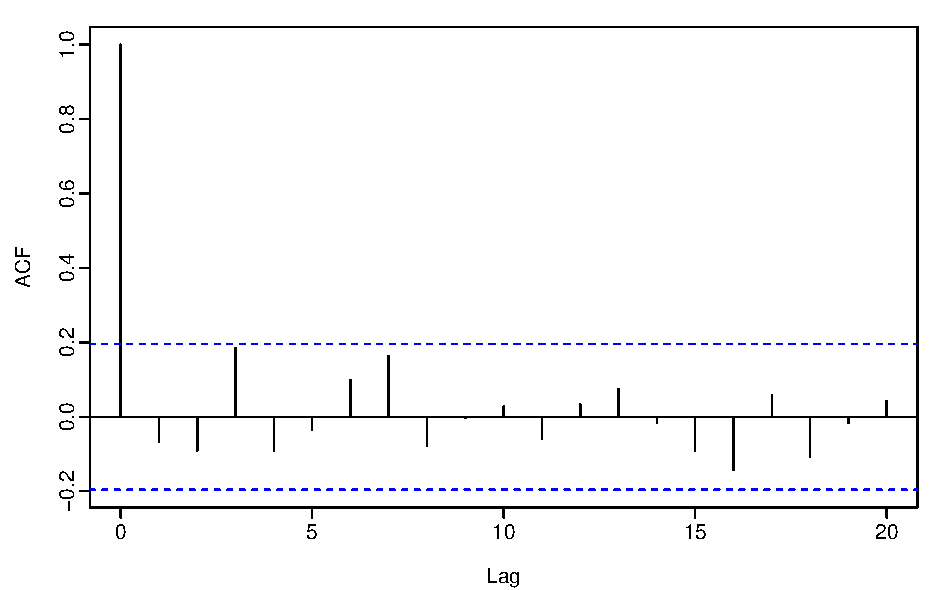
\includegraphics{chp2_acf80}
\caption[Correlogram of auto-correlations]{Correlogram of AirPassenger data a built-in data set of R, over a range of time lags from 1 to 80.}
\label{fig:acf80}
\end{figure}

%\begin{figure}[tbph!]
%\centering
%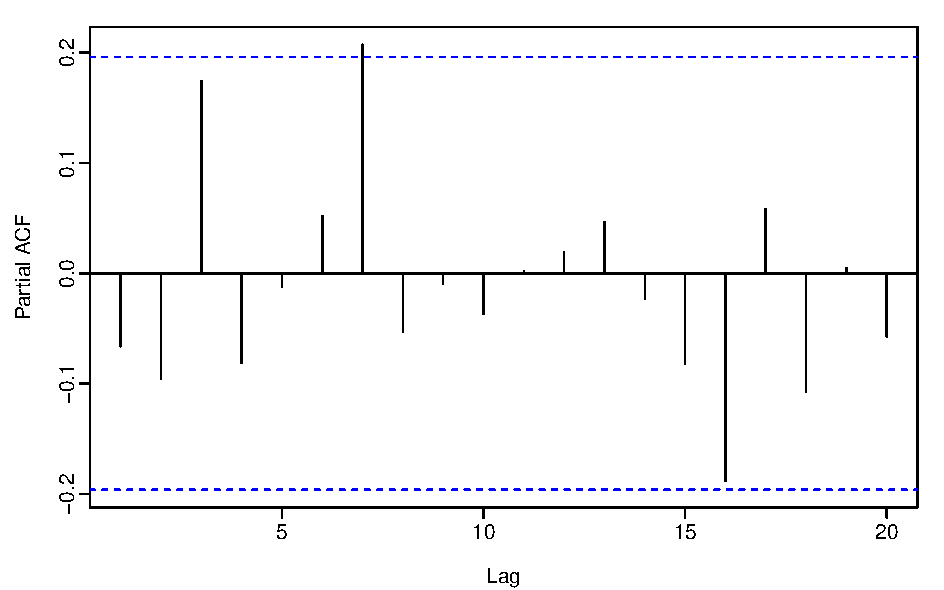
\includegraphics{chp2_p_pacf}
%\caption[Correlogram of a seasonal component]{Correlogram of the seasonal component of the AirPassenger data, a built-in data set of R, over a range of time lags from 1 to 80.}
%\label{fig:pacf}
%\end{figure}

The partial correlation is defined as the degree of correlation not already explained by the correlations previously measured. If the regression of variable A on variables B1, B2 and B3 is considered the partial correlation between variables A and B3 is the degree of correlation not accounted for by their common correlations with variables B1 and B2. In a similar manner the partial autocorrelation is the unexplained correlation after considering the variable and itself at an earlier time period. In a series, if a variable A at time t is correlated with an earlier lag at time t-1 it follows that the variable at t-1 itself is correlated with the previous variable at lag t-2. By extension the variable at time t should also be correlated with the variable at lag t-2, as the correlation will propagate through the series. The partial autocorrelation is the difference the expected correlations due the propagating factors and the actual correlation measured.

\label{todo3}
The lag at which the PAC tails off can be a good candidate for the AR aspect, looking at Figure \ref{fig:correlogram} this is three - ARMA(3,0)

The AC indicates potential values for the MA component, looking at Figure \ref{fig:acf80} this is one - ARMA(0,1)

A third alternative is an ARMA(p,q) as both the AC and PAC tail off to zero.

Generally one would start with the simplest model so an ARMA(0,1) should be a good place to start the modelling.

\subsection{Hybrid Models}
Auto-regressive (integrated) moving average models have shown themselves to be important modelling methods for time series data, including financial time series data. However the techniques have limitations that have detracted from their popularity, namely their assumption of a linear relationship and the need for a lot of data to produce accurate results. In order to address these limitations a variety of hybrid solutions have been proposed in which ARIMA models are combined with other techniques, often non-linear prediction algorithms \citep{Wang2012758,Khashei20124344,Aladag20091467}.

% ARIMA / ANNs
One combination that has found a lot of attention in the literature is the combination of Artificial Neural Networks (ANNs) with ARIMA. \cite{Khashei2009956} report on the use of this combination in a attempt to predict the future price movement in gold and US dollar / Iran rials financial markets. The workers report favourable results in comparison to the techniques alone and suggest the method as having potential for accurate predictions of non-linear time series data. In a similar study \cite{Zhang2003159} applied a combination of ARIMA and ANN to various data sets including the British pound / US dollar exchange rate. They observe that in the literature in general these two popular techniques are frequently compared in terms of predictive power with the reported results non-conclusive. Results from the three data sets modelled show that the combination of the two methods outperform the individual ones when the mean squared error (MSE) and mean
absolute deviation (MAD) are used as the measure of forecasting accuracy.

\cite{Fatima20082742} also investigated the impact of a hybrid approach in modelling short term predictions for the Karachi Stock Exchange index (KSE100). The authors reported comparison results for ANN versus ARIMA and a hybrid of ANN/ARIMA. The hybrid solution out-performed the individual ARIMA and ANN models. It is postulated that a rationale for this is that at any point in time financial markets are subject to linear, non-linear and volatility patterns as the cumulative effects of government fiscal and monetary policies and general rumour and political instabilities feed into the market. Under these complex conditions simple models can only capture one aspect of the underlying factors affecting the price series. A hybrid combination approach is more successful as more of the market variance is modelled.

% ARIMA / WAVELETS
\cite{Kriechbaumer201432} reports on a further hybrid approach to forecast the prices of aluminum, copper, lead and zinc. Previous research has indicated that these markets exhibit a strong cyclic behaviour. In an attempt to factor this into the predictive model ARIMA was coupled with a wavelet approach. Wavelet analysis decomposes a time series into its frequency and time domains in an attempt to isolate this cyclic behaviour. The performance of the ARIMA modelling was shown to be enhanced substantially by the addition of wavelet based multi-resolution analysis (MRA) before performing the ARIMA analysis.

\cite{Tan20103606} have also reported the combination of wavelet analysis and ARIMA in the prediction of electricity prices. The general method employed is to transform the original time series data set into a collection of sub-series through the application of wavelet analysis. Subsequent to the transformation a prediction for each sub-series can be made with ARIMA modelling. The final forecasted result is obtained by reforming the sub-series back into the original time series. The authors report resulting showing the enhanced predictive power of the ARIMA wavelet hybrid approach compared to ARIMA and GARCH models used in isolation.

% ARIMA / SVM
\cite{Pai2005497} reported on attempts to overcome the limitation of ARIMA models in that the time series must be linear by use of an hybrid ARIMA / Support vector machine (SVMs) combination. SVMs have been successfully applied to to non-linear regression problems and the authors have harnessed the strengths of both methodologies in order to predict the prices of a selection of fifty stocks. Results from the work show that the hybrid method out-performs the ARIMA and SVM methods individually.

\cite{Rout20147} report the use of ARMA models in the prediction of exchange rates. The workers note the limitations of ARMA in that the time series data must be linear and stationary, a condition often not met in practical situations and the difficulty in deriving steps one and two (listed previously) in developing the ARMA model. In order to overcome these limitations ARMA is combined with differential evolution (DE) in order to determine the models feed-forward and feed-back parameters. The results from the prediction models generated are compared with models resulting from ARMA in conjunction with particle swarm optimisation (PSO), cat swarm optimisation (CSO), bacterial foraging optimization (BFO) and forward backward least mean square (FBLMS). The workers conclude that the ARMA - DE model produces the best short and long-range predictions from the options tested and is a potentially valuable method in predicting exchange rates on the international finance markets.

%ARIMA/GARCH
%34 - International evidence on crude oil price dynamics: Applications of ARIMA-GARCH models - \cite{Mohammadi20101001}

%20 - Forecasting aggregate retail sales:: a comparison of artificial neural networks and traditional methods - \cite{Alon2001147}
%Looks at various time series models, good overview.
 
%\subsection{Seasonality}

%28 -Dynamic seasonality in time series - \cite{So2014212}

%\subsection{Data Mining of Time Series Data}
%21 - A review on time series data mining - \cite{Fu2011164}
%%Time series is an important class of temporal data objects and it can be easily obtained from scientific and financial applications. A time series is a collection of observations made chronologically. The nature of time series data includes: large in data size, high dimensionality and necessary to update continuously. Moreover time series data, which is characterized by its numerical and continuous nature, is always considered as a whole instead of individual numerical field. The increasing use of time series data has initiated a great deal of research and development attempts in the field of data mining. The abundant research on time series data mining in the last decade could hamper the entry of interested researchers, due to its complexity. In this paper, a comprehensive revision on the existing time series data mining research is given. They are generally categorized into representation and indexing, similarity measure, segmentation, visualization and mining. Moreover state-of-the-art research issues are also highlighted. The primary objective of this paper is to serve as a glossary for interested researchers to have an overall picture on the current time series data mining development and identify their potential research direction to further investigation.


%\subsubsection{Neural Nets}
%
%I. Kaastra, M. Boyd, Designing a neural network for forecasting financial and
%economic time-series, Neurocomputing 10 (1996) 215–236.
%
%3 - The use of data mining and neural networks for forecasting stock market returns - \cite{Enke2005927}
%%
%6 - Intelligent technical analysis based equivolume charting for stock trading using neural networks - \cite{Chavarnakul20081004}
%
%23 - A neural-network-based nonlinear metamodeling approach to financial time series forecasting - \cite{Yu2009563}

%\subsubsection{SVM}
%5 - Forecasting stock market movement direction with support vector machine - \cite{Huang20052513}
%
%7 - Financial time series forecasting using support vector machines - \cite{Kim2003307}
%
%\subsubsection{SOM}
%8 - A two-stage architecture for stock price forecasting by integrating self-organizing map and support vector regression - \cite{Hsu20097947}
%%
%9 - A hybrid procedure for stock price prediction by integrating self-organizing map and genetic programming - \cite{Hsu201114026}
% 
%\subsubsection{Clustering}
%10 - Clustering of financial time series - \cite{DUrso20132114}
%
%22 - Clustering of time series data—a survey - \cite{WarrenLiao20051857}
%
%%
%%\subsubsection{Decision Trees}
%%
%11 - Trend discovery in financial time series data using a case based fuzzy decision tree " - \cite{Chang20116070}
%%
%%
%12 - Evolving and clustering fuzzy decision tree for financial time series data forecasting "  - \cite{Lai20093761}

%\subsection{ARCH/GARCH}
%
%ARCH introduced by \cite{Engle} 
%
%GARCH introduced in \cite{TaylorGARCH}
%
%GARCH survey \cite{BollerslevGARCH}



%12 - A nonparametric GARCH model of crude oil price return volatility " - \cite{Hou2012618}
%
%"Volatility in crude oil futures: A comparison of the predictive ability of GARCH and implied volatility models " - \cite{Agnolucci2009316}

%\subsection{Hybrid Approaches}
%
%24 - A new class of hybrid models for time series forecasting - \cite{Khashei20124344}
%
%25 - An artificial neural network (p, d, q) model for timeseries forecasting - \cite{Khashei2010479}
%
%26 - Forecasting nonlinear time series with a hybrid methodology - \cite{Aladag20091467}
%
%27 - Stock index forecasting based on a hybrid model " - \cite{Wang2012758} - GOOD

%\subsection{Comparison of Approches}
%
%AR - 30 - Forecasting models for interval-valued time series " - \cite{Maia20083344}
%
%Neural network and traditional time series
%techniques have been compared in several studies. Sharda
%and Patil [29] found that neural networks performed as good as
%the automatic Box–Jenkins procedure. Maier and Dandy [23]
%suggest that the ARIMA model is better suited for short-term
%forecasts and that neural networks are better suited for longerterm
%forecasts.
%
%R. Sharda, R. Patil, Neural networks as forecasting exports: an empirical test,
%in: Proceedings of IJCNN Meeting 1990 2, 1990, pp. 491–494.
%
%H.R. Maier, G.C. Dandy, Neural network models for forecasting univariate time
%series, Neural Networks World 6 (5) (1996) 747–772.


%\subsubsection{Commodities}
%12a - Forecasting volatility of crude oil markets " - \cite{Kang2009119}
%%
%14 - Modeling and forecasting petroleum futures volatility " - \cite{Sadorsky2006467}



